\documentclass[11pt,a4paper]{report}
\usepackage{graphicx,color}
\usepackage[english]{babel}
\usepackage[english]{tuereport2008}
\usepackage{booktabs}

\graphicspath{{images/}}

\title{Visualizing the Netherlands}
\subtitle{Manual}
\author{Michiel Fortuin\\Wouter Lok}
\version{2.0}
\orderissuer{}
\copyholder{}
\administrativeunit{Department of Mathematics and Computer Science}   % insert department name here
\department{Visualization}     % subdepartment, or group
\website{}
\reference{}

\begin{document}
\maketitle

\chapter{Manual}
\begin{figure}[htb!]
    \centering
    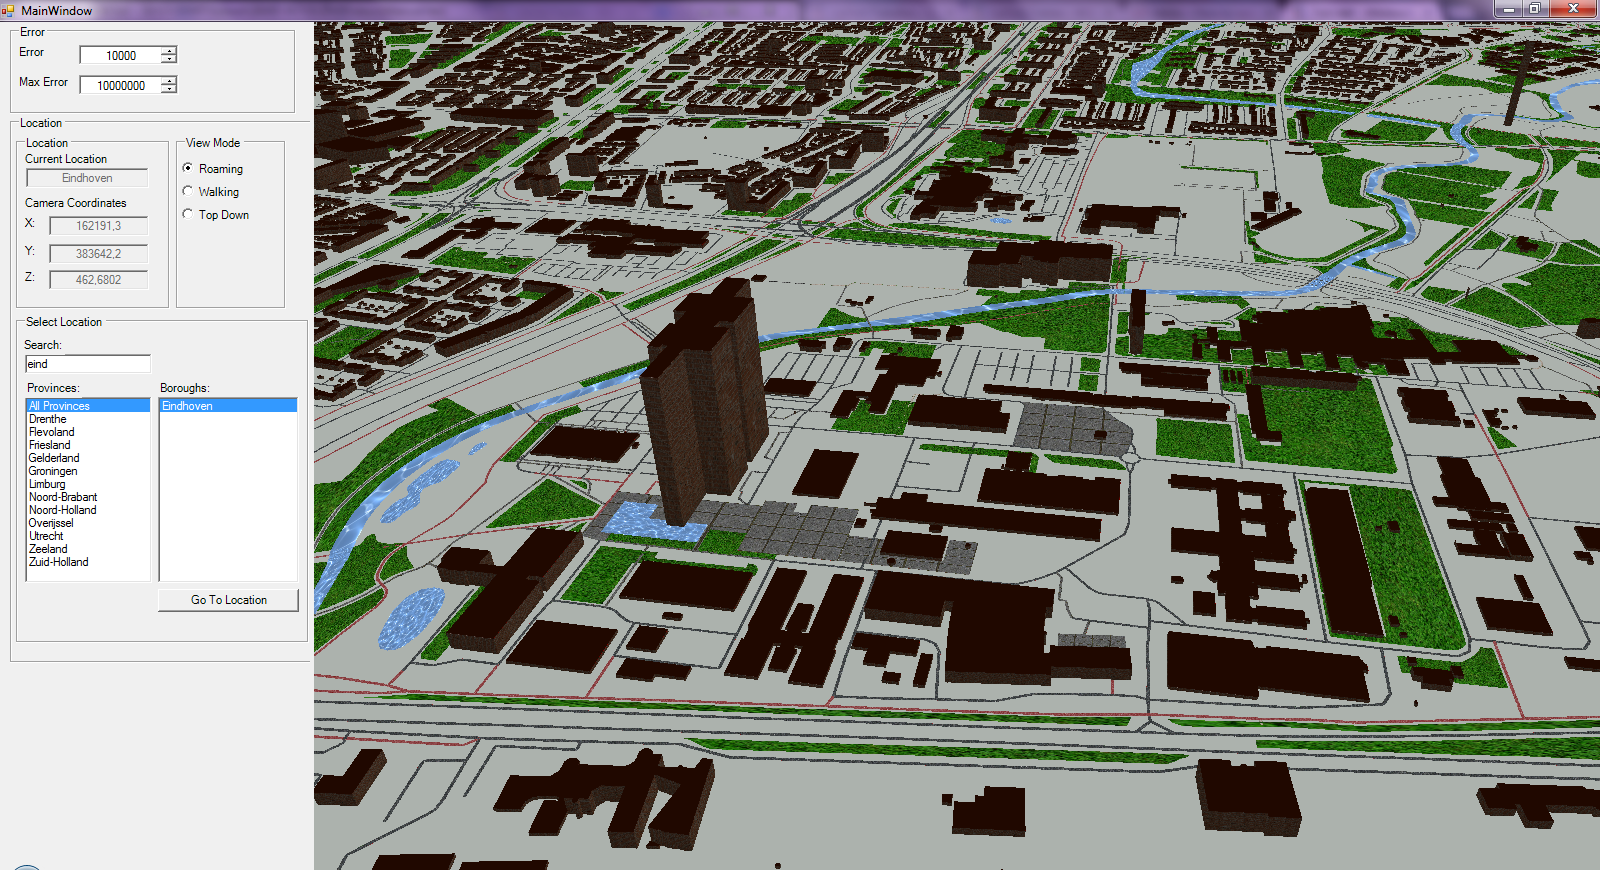
\includegraphics[width=0.9\textwidth]{ManualImage}
    \caption{Screenshot}
    \label{fig:Screenshot}
\end{figure}

In image \ref{fig:Screenshot} a screenshot of the application is shown. Below is a list (table \ref{tab:descriptionItems}) with the meaning of the controls on the screen. In table \ref{tab:controls} there is a list of keyboard and mouse controls to change the view. To start up the application use the shortcut ''Visualize Eindhoven''. This shortcut adds the dataset path as parameter to the application.

% Table generated by Excel2LaTeX from sheet 'Sheet2'
\begin{table}[htbp]
  \centering
  \caption{Description of application items}
    \begin{tabular}{lp{10cm}}
    \toprule
    Item  & Description \\
    \toprule
    Error & The error that is added for every meter. Higher error means a lower image quality. \\\midrule
    Max Error & The maximum error that is loaded. This is also the maximum drawing distance. \\\midrule
    Current Location & The current borough location. \\\midrule
    Camera Coordinates & The current coordinate system. The unit is in meters and the Rijksdriehoekscoördinaten system is used. \\\midrule
    View mode & The viewmode \\\midrule
    * Roaming & A simple flying camera. \\\midrule
    * Walking & A camera that stays on a height of 1.75 meter. \\\midrule
    * Top Down & A top view of the area. \\\midrule
    Search & A way to search in the boroughs list. \\\midrule
    Provinces & A list with provinces. With it, it's possible to filter the boroughs list. \\\midrule
    Boroughs & A list with boroughs. (see Go To Location) \\\midrule
    Go To location & Transport to the location of the currently selected boroughs. \\
    \bottomrule
    \end{tabular}%
  \label{tab:descriptionItems}%
\end{table}%



% Table generated by Excel2LaTeX from sheet 'Sheet1'
\begin{table}[htbp]
  \centering
  \caption{Controls}
    \def\buttonsize{0.1}
    \begin{tabular}{rr}
    \toprule
          Control & Action \\
    \toprule
          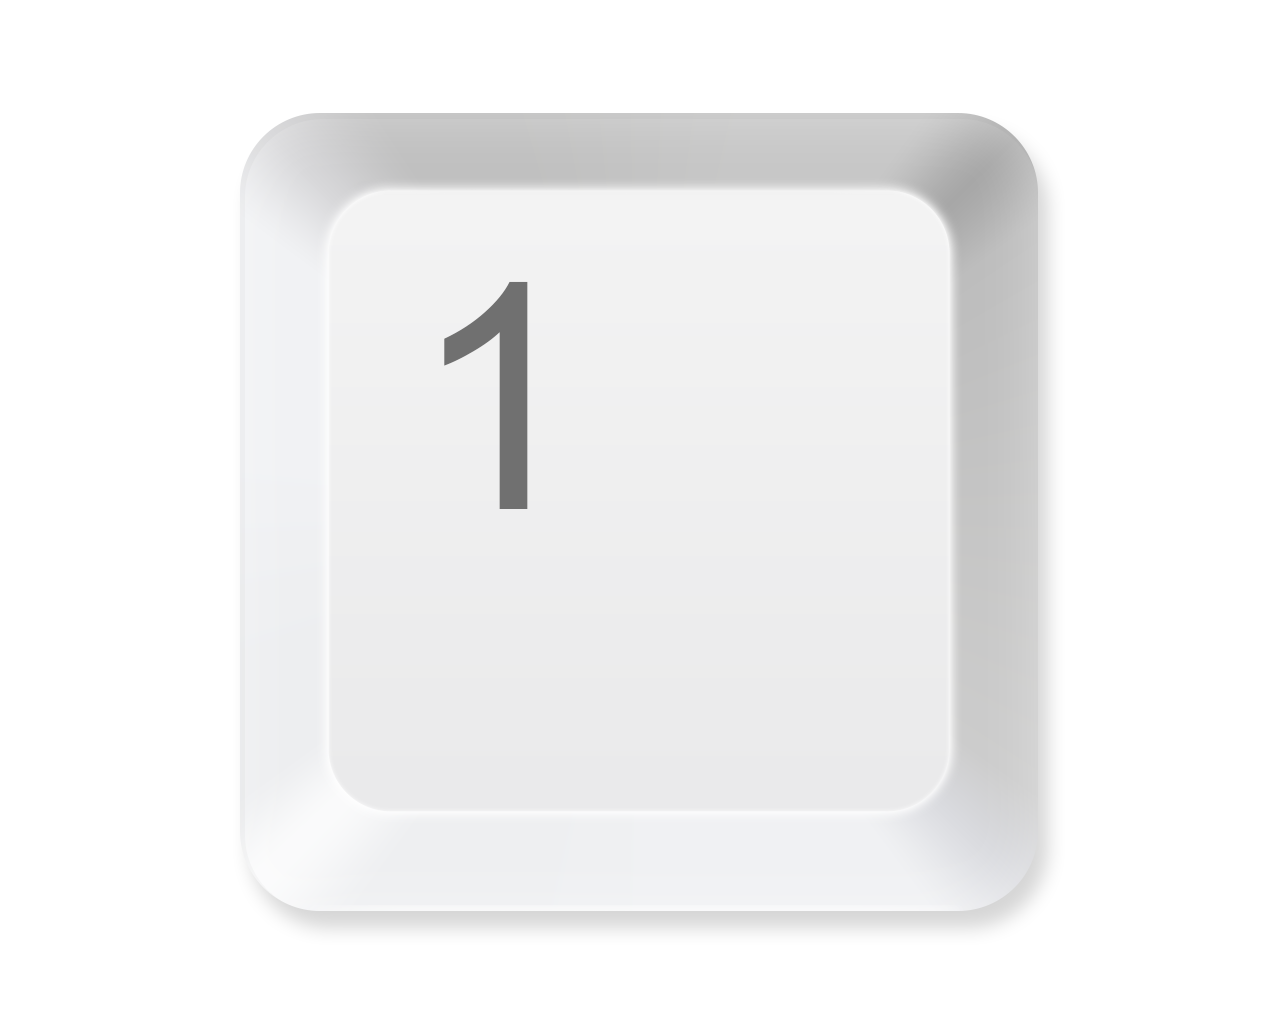
\includegraphics[width=\buttonsize\textwidth]{Button1} & Speed 1 (slowest)\\
    \midrule
          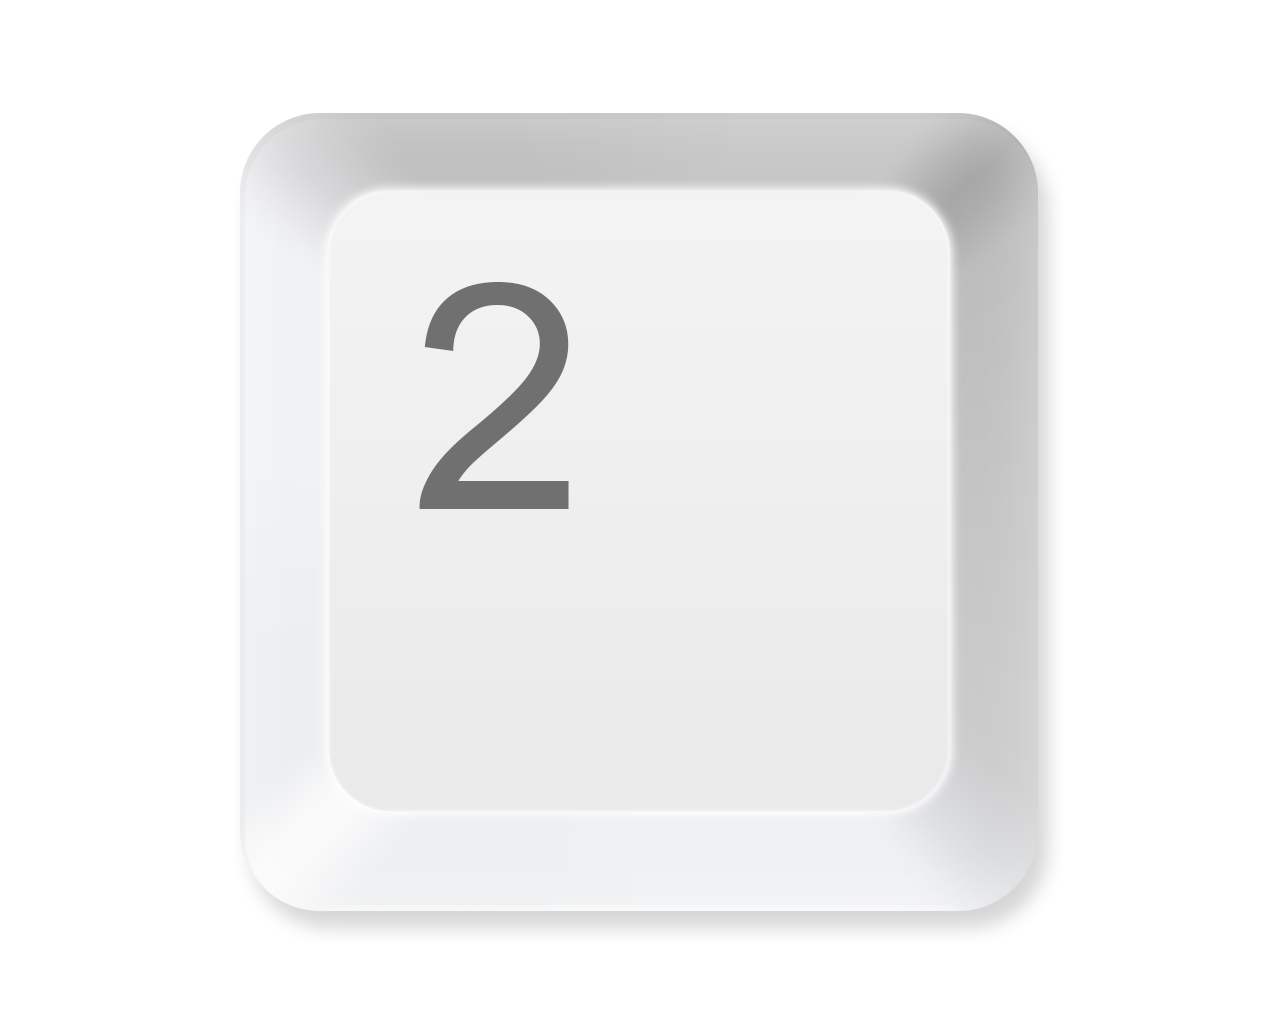
\includegraphics[width=\buttonsize\textwidth]{Button2} & Speed 2 \\
    \midrule
          & Speed 3 .. 8  \\
    \midrule
          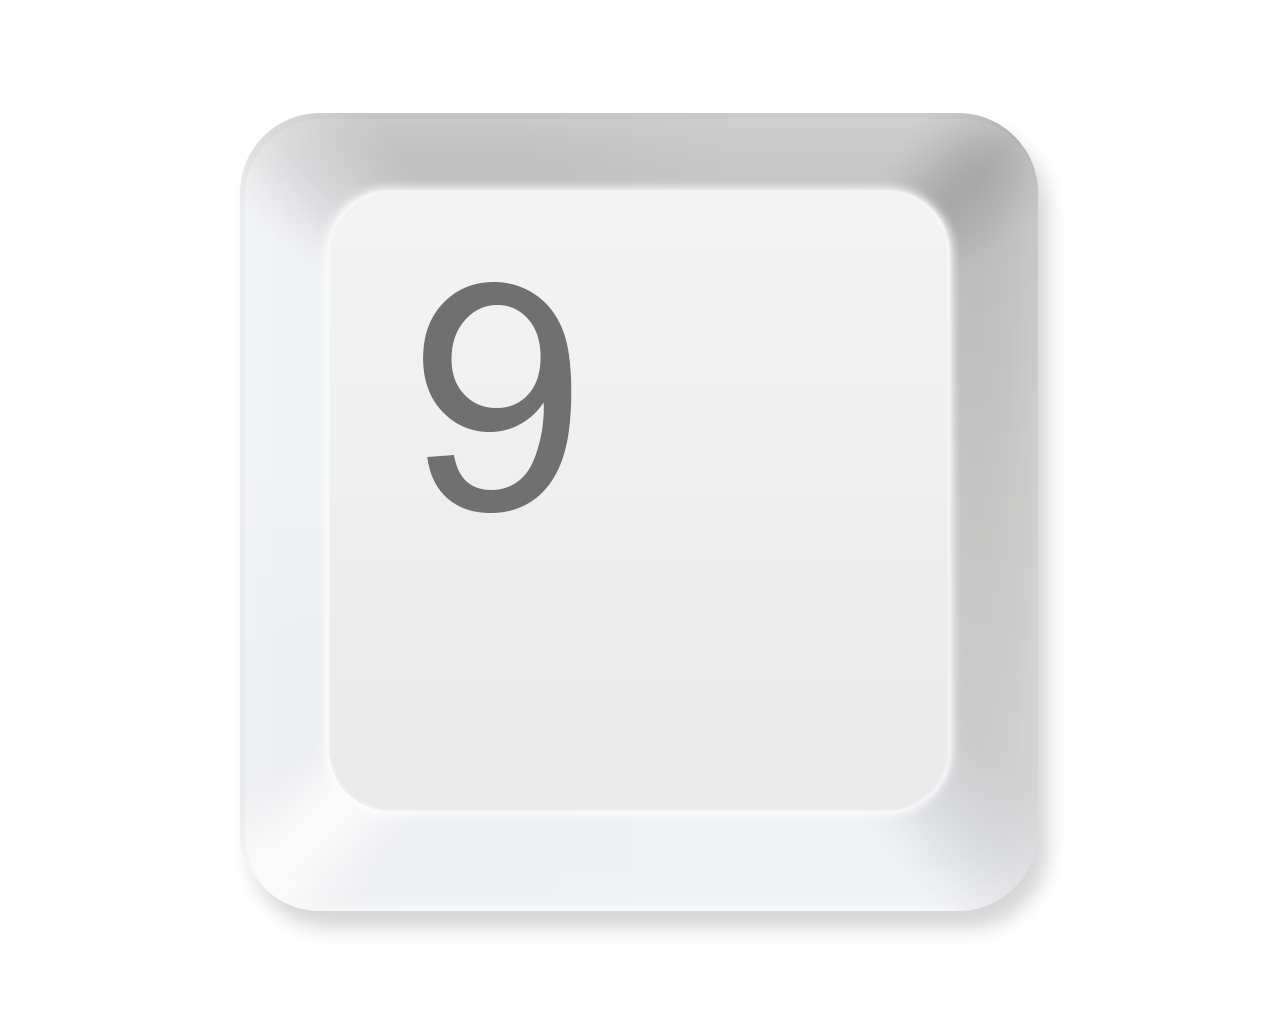
\includegraphics[width=\buttonsize\textwidth]{Button9} & Speed 9 \\
    \midrule
          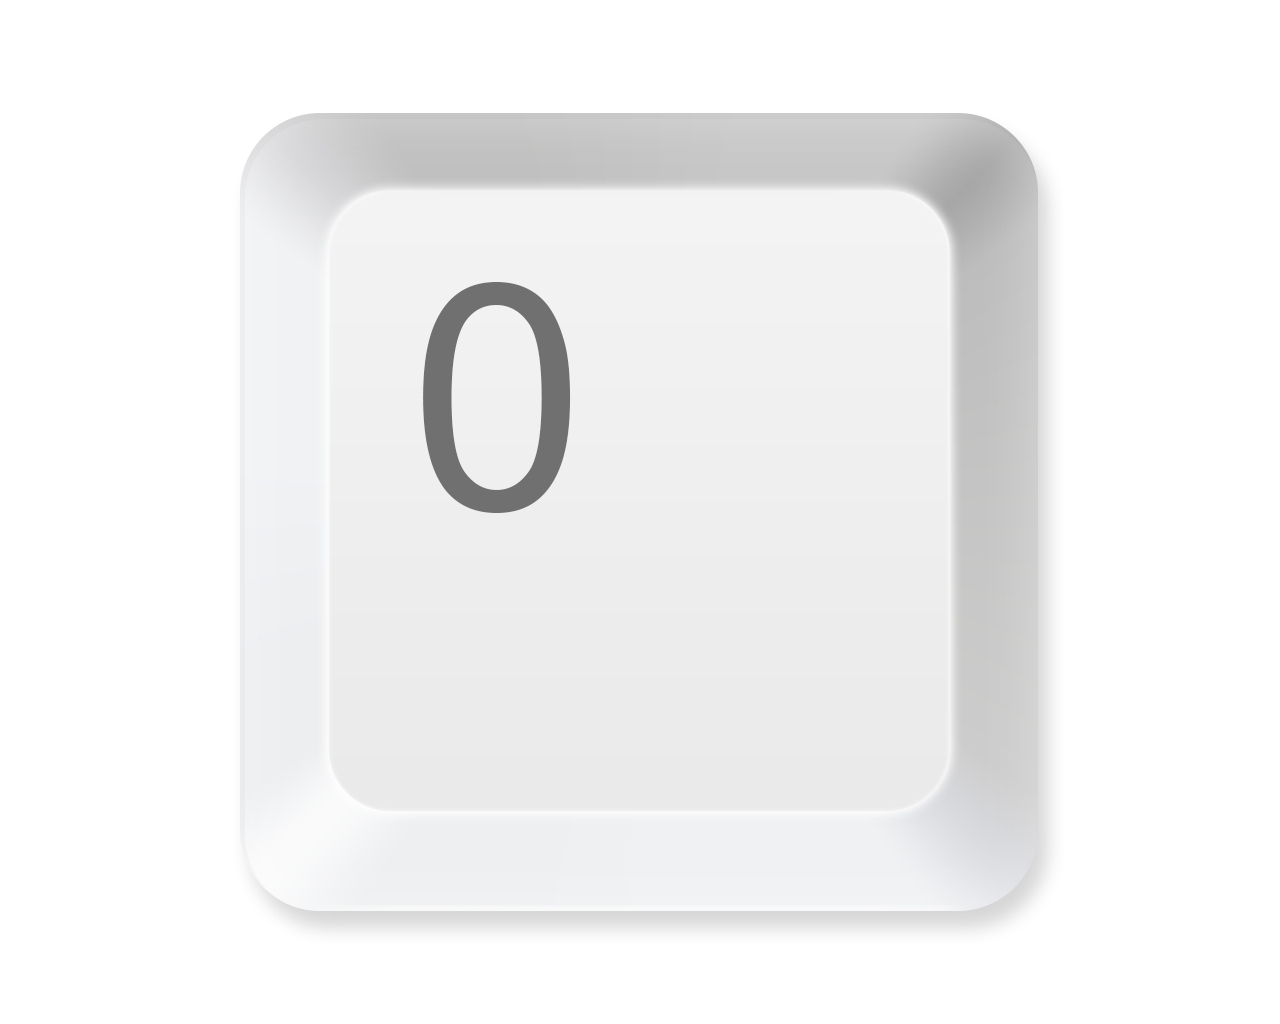
\includegraphics[width=\buttonsize\textwidth]{Button0} & Speed 0 (fastest)\\
    \midrule
          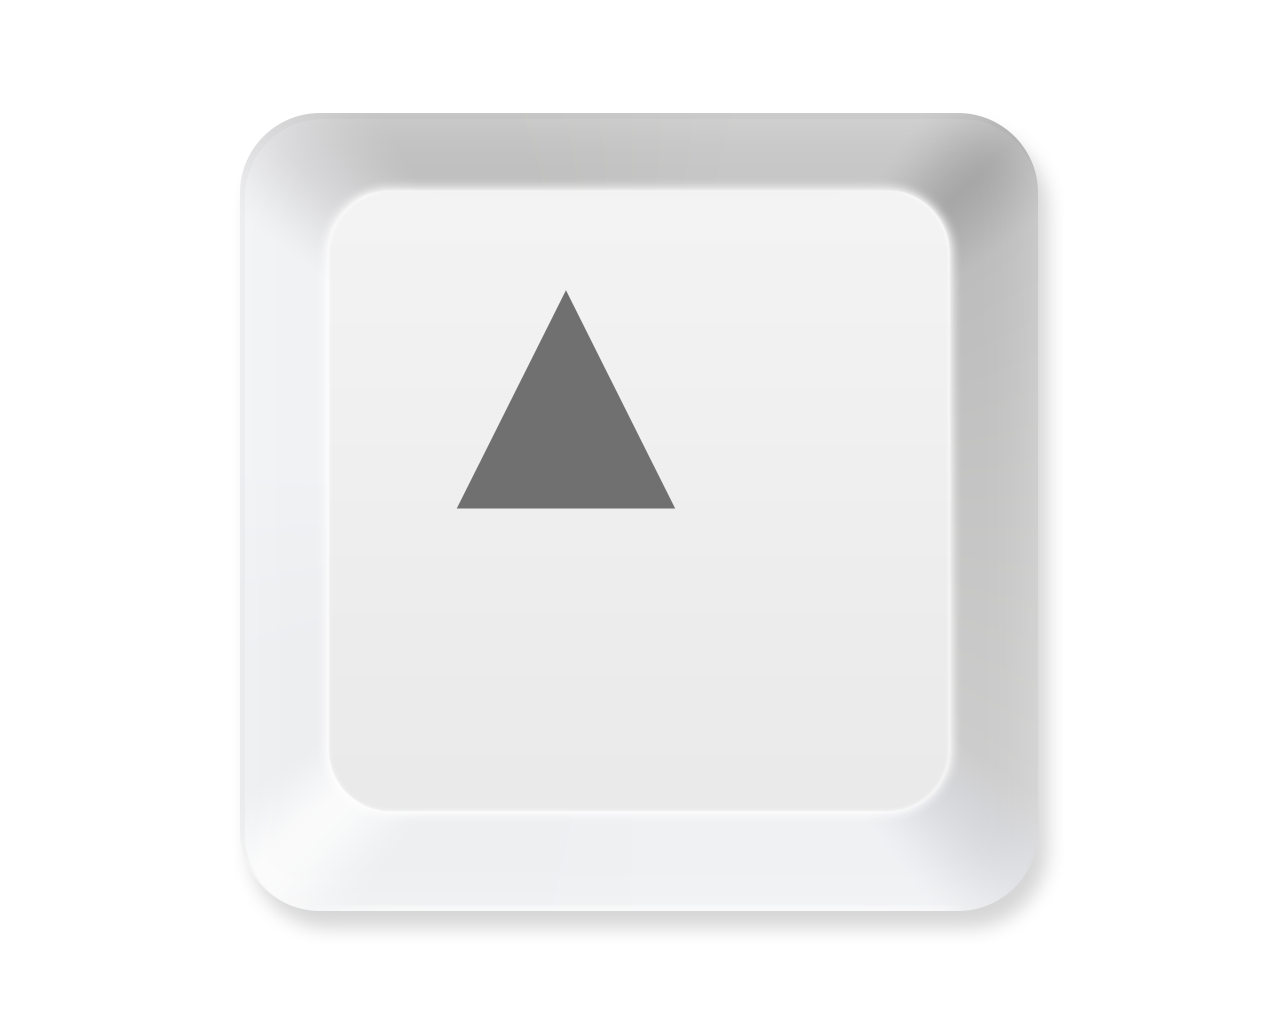
\includegraphics[width=\buttonsize\textwidth]{ButtonUp}
\includegraphics[width=0.1\textwidth]{ButtonW} & Forward \\
    \midrule
          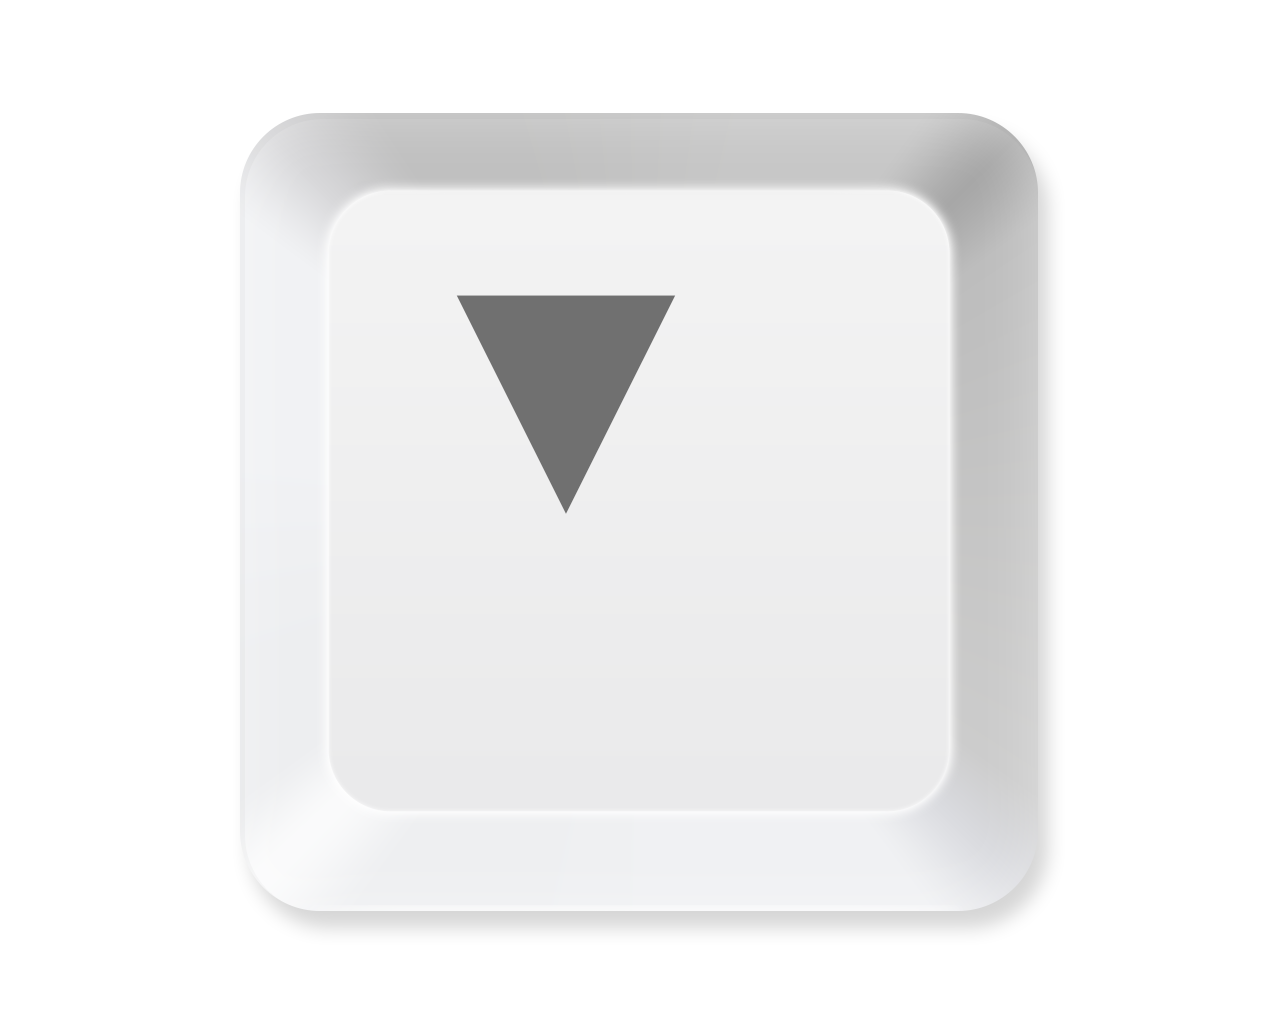
\includegraphics[width=\buttonsize\textwidth]{ButtonDown}
\includegraphics[width=0.1\textwidth]{ButtonS} & Backward \\
    \midrule
          
\includegraphics[width=\buttonsize\textwidth]{ButtonLeft}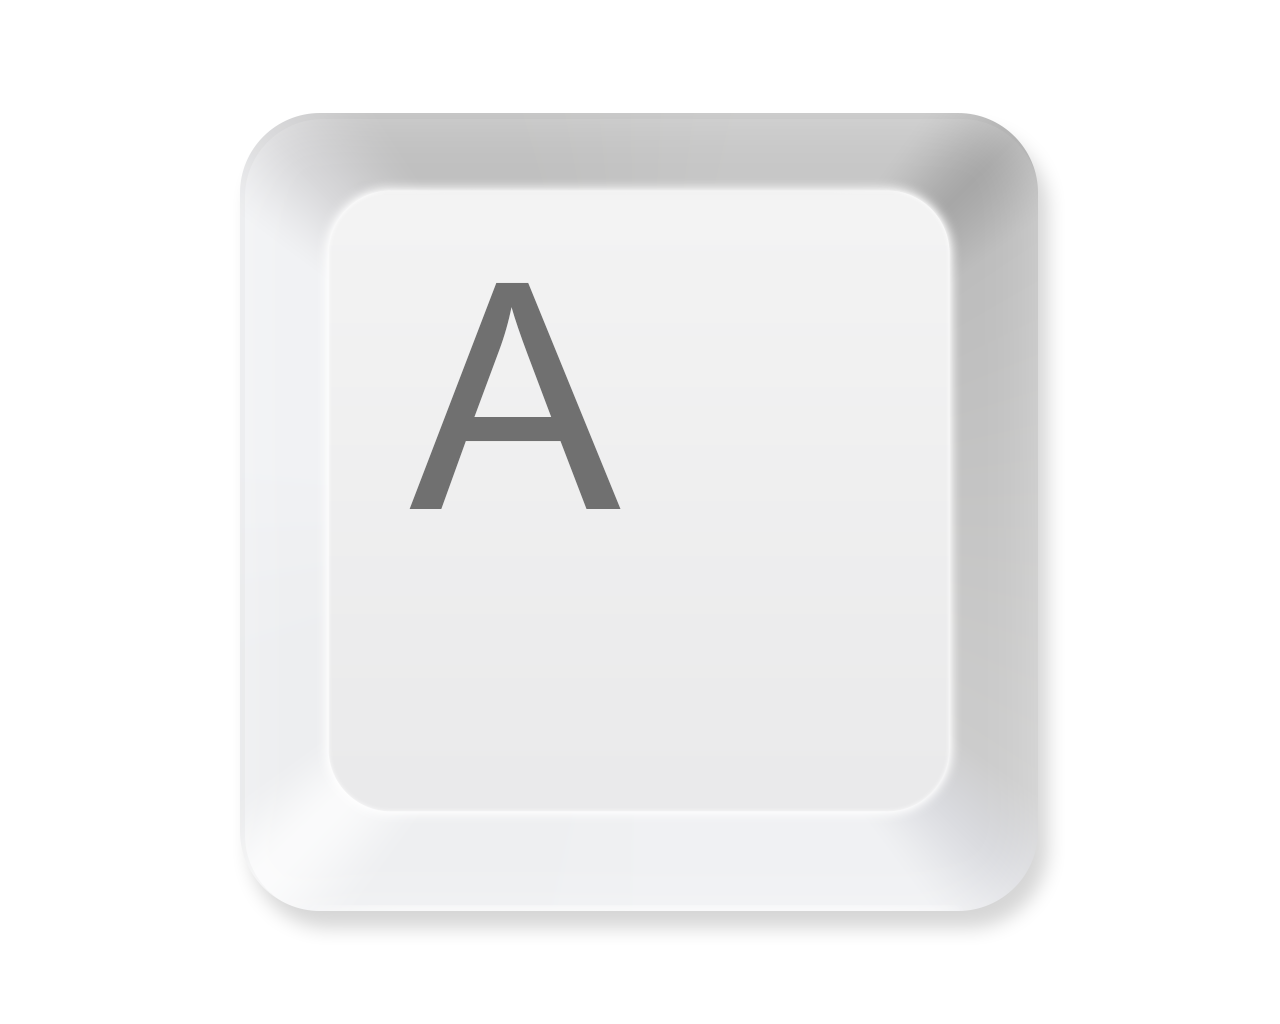
\includegraphics[width=0.1\textwidth]{ButtonA} & Strafe left \\
    \midrule
          
\includegraphics[width=\buttonsize1\textwidth]{ButtonRight}
\includegraphics[width=0.1\textwidth]{ButtonD} & Strafe right \\
    \midrule
          
\includegraphics[width=\buttonsize\textwidth]{ButtonSpace} & Change view \\
    \midrule
          
\includegraphics[width=\buttonsize\textwidth]{ButtonQ} & Zoom in \\
    \midrule
          
\includegraphics[width=\buttonsize\textwidth]{ButtonE} & Zoom out \\
    \midrule
          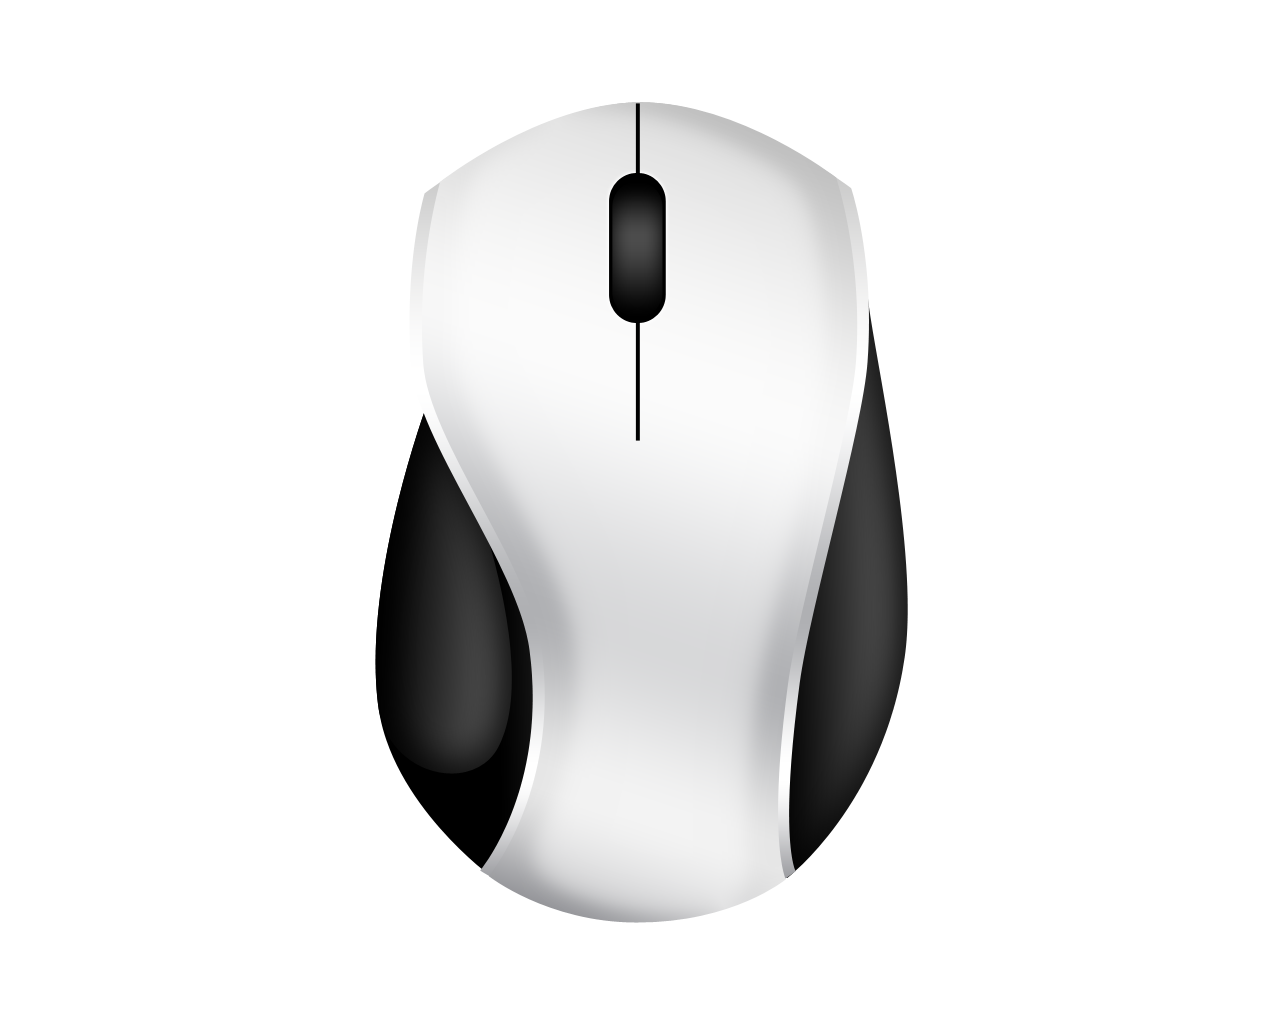
\includegraphics[width=\buttonsize\textwidth]{ButtonMouse} + button & Rotate view \\
    \bottomrule
    \end{tabular}%
  \label{tab:controls}%
\end{table}%


\end{document} 